% =====================================================================
% Final-project presentation deck
%
% Compile with:
%   pdflatex final_presentation.tex
%   pdflatex final_presentation.tex
%
% Output: final_presentation.pdf  (10 slides, 16:9)
% =====================================================================
\documentclass[aspectratio=169,12pt]{beamer}

\usetheme{default}
\setbeamertemplate{navigation symbols}{}
\setbeamertemplate{itemize items}[circle]
\setbeamertemplate{itemize subitem}[triangle]

\usepackage{graphicx}
\usepackage{booktabs}
\usepackage{xcolor}
\usepackage{tikz}
\usepackage{array}
\usepackage{tabularx}
\usepackage{colortbl}
\usepackage{lmodern}
\usepackage[T1]{fontenc}
\usepackage{microtype}

% --- modern color palette (clean, professional) ---
\definecolor{primary}{HTML}{1A365D}      % deep navy
\definecolor{accent}{HTML}{D97706}        % warm orange (high contrast)
\definecolor{ok}{HTML}{059669}            % success green
\definecolor{warn}{HTML}{B91C1C}          % warn red
\definecolor{soft}{HTML}{F1F5F9}          % light grey for table headers
\definecolor{ink}{HTML}{1F2937}           % body text
\definecolor{muted}{HTML}{6B7280}         % subtle grey

% --- frame styling ---
\setbeamercolor{normal text}{fg=ink, bg=white}
\setbeamercolor{frametitle}{fg=white, bg=primary}
\setbeamercolor{title}{fg=primary}
\setbeamercolor{subtitle}{fg=accent}
\setbeamercolor{itemize item}{fg=primary}
\setbeamercolor{itemize subitem}{fg=accent}
\setbeamerfont{frametitle}{series=\bfseries, size=\Large}
\setbeamerfont{normal text}{size=\normalsize}

% Full-width navy frame title bar
\setbeamertemplate{frametitle}{%
  \nointerlineskip%
  \begin{beamercolorbox}[wd=\paperwidth, sep=0.5cm, ht=0.95cm]{frametitle}%
    \strut\insertframetitle\strut%
  \end{beamercolorbox}%
}

% Generous spacing
\setlength{\parskip}{0.5em}
\renewcommand{\arraystretch}{1.5}

\newcommand{\hi}[1]{{\color{accent}\textbf{#1}}}      % accent highlight
\newcommand{\hp}[1]{{\color{primary}\textbf{#1}}}     % primary highlight

% --- title page ---
\title{Loan Default Prediction}
\subtitle{Comparing Classic ML and Neural Networks under Class Imbalance}
\author{Minwoo Yoo \and Nathaniel Badalov}
\date{}

% =====================================================================
\begin{document}
% =====================================================================

% --------------------------- Slide 1 — Title ---------------------------
{
  \setbeamertemplate{frametitle}{}
  \begin{frame}
    \vspace{1.4cm}
    \begin{center}
      {\color{primary}\Huge\bfseries Loan Default Prediction}\\[0.8em]
      {\color{accent}\large Comparing Classic ML and Neural Networks \\[0.2em] under Class Imbalance}\\[2.4em]
      \rule{0.35\textwidth}{0.6pt}\\[1em]
      {\large Minwoo Yoo \quad·\quad Nathaniel Badalov}\\[0.6em]
      {\color{muted}\textit{Home Credit Default Risk · Kaggle}}
    \end{center}
  \end{frame}
}

% --------------------------- Slide 2 — Problem ---------------------------
\begin{frame}{Problem \& Motivation}
  \vspace{0.4em}

  \hp{The task}\\[0.3em]
  Predict the probability that a loan applicant defaults
  (binary classification, \texttt{TARGET}~$\in \{0, 1\}$).

  \bigskip\bigskip
  \hp{Why this matters}
  \begin{itemize}
    \item Lenders need accurate risk scoring to balance approval volume and credit losses.
    \item False negatives cost the full unpaid principal — far more than the foregone interest of a false positive.
  \end{itemize}

  \bigskip
  \hp{The challenge: class imbalance}
  \begin{itemize}
    \item Only $\sim$\hi{8.07\%} of applicants default — the data is severely imbalanced.
    \item A naive ``always predict no default'' baseline scores 92\% accuracy with \hi{zero recall}.
    \item Accuracy alone is misleading; we use \hi{ROC AUC} as the primary metric.
  \end{itemize}

  \bigskip
  \hp{Research question}
  \begin{center}
    {\color{accent}\itshape\Large Do classic shallow learners and neural networks\\
    respond differently to class imbalance handling?}
  \end{center}
\end{frame}

% --------------------------- Slide 3 — Dataset ---------------------------
\begin{frame}{Dataset · Home Credit Default Risk}
  \vspace{0.3em}
  \begin{columns}[T,onlytextwidth]
    \column{0.50\textwidth}
      \hp{Size}
      \begin{itemize}
        \item Train: \hi{307{,}511} applicants $\times$ 122 features
        \item Test: 48{,}744 applicants  (Kaggle hidden labels)
      \end{itemize}

      \bigskip
      \hp{Class imbalance}
      \begin{itemize}
        \item Default rate $\approx$ \hi{8.07\%}\\
              (24{,}825 / 307{,}511)
      \end{itemize}

      \bigskip
      \hp{Strongest signals}
      \begin{itemize}
        \item \texttt{EXT\_SOURCE\_1/2/3}\\
              external credit scores ($|\rho|\!\approx\!0.16$--$0.18$)
        \item \texttt{DAYS\_EMPLOYED}\,$=\,$365{,}243\\
              sentinel for unemployed (18\%)
        \item Building-info columns: 50--70\% missing
      \end{itemize}

    \column{0.48\textwidth}
      \vspace{1.0em}
      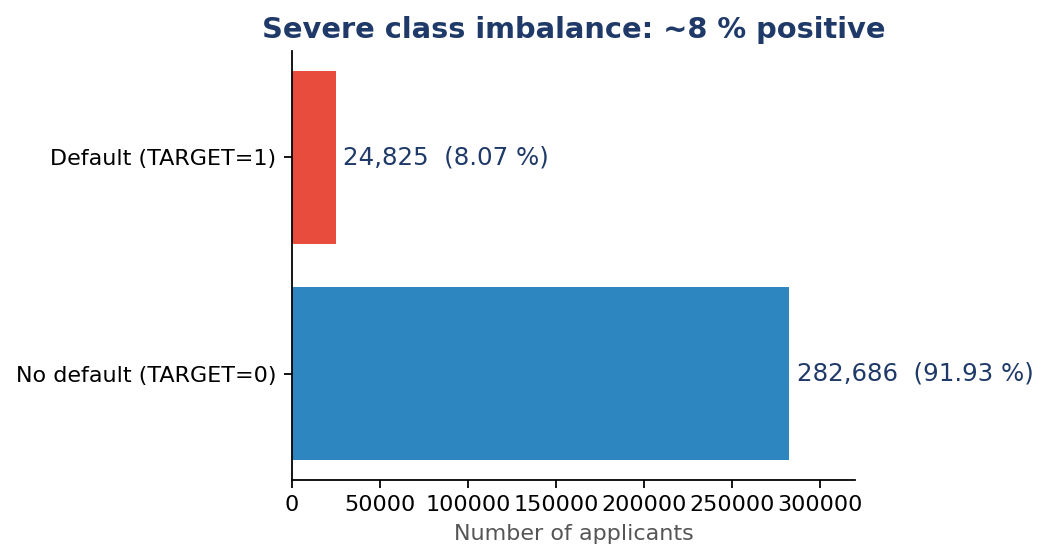
\includegraphics[width=\linewidth]{../result/home_credit/figure/class_balance.png}
  \end{columns}
\end{frame}

% --------------------------- Slide 4 — Shared Pipeline ---------------------------
\begin{frame}{Shared Pipeline}
  \vspace{0.3em}
  \hp{Preprocessing  \small\textit{— identical for all five models}}
  \begin{itemize}
    \item \hi{80/20 stratified} train--val split  (\texttt{random\_state = 42})
    \item Drop \texttt{SK\_ID\_CURR}; keep IDs only for the submission file
    \item Mean imputation for numeric NaN; one-hot encode 16 categoricals $\to$ \hi{244 features}
    \item \texttt{StandardScaler} fitted on train only  (essential for LR / MLP)
  \end{itemize}

  \bigskip\bigskip
  \hp{Tuning \& validation}
  \begin{itemize}
    \item \texttt{GridSearchCV} with \texttt{PredefinedSplit}  (single train$\to$val fold)
    \item Scoring: \texttt{roc\_auc}; best parameter setting picked per model
    \item CV CSVs saved to \texttt{result/home\_credit/cv\_results/GridSearchCV/}
  \end{itemize}
\end{frame}

% --------------------------- Slide 5 — Classic ML Models ---------------------------
\begin{frame}{Classic ML Models}
  \vspace{0.2em}
  \begin{columns}[T,onlytextwidth]
    \column{0.62\textwidth}
      \hp{Logistic Regression}\hfill val AUC \hi{0.7487}\\[0.2em]
      \small \texttt{C} $\in \{0.01, 0.1, 1, 10\}$, \, \texttt{tol} $\in \{10^{-5}, 10^{-4}, 10^{-3}\}$\\
      \texttt{class\_weight=balanced}
      \medskip

      \hp{Random Forest}\hfill val AUC \hi{0.7470}\\[0.2em]
      \small \texttt{n\_estimators} $\in \{100, 200\}$\\
      \texttt{min\_samples\_split} $\in \{2, 20, 100\}$\\
      \texttt{min\_samples\_leaf} $\in \{1, 20, 100\}$,\, \texttt{class\_weight=balanced}
      \medskip

      \hp{HistGradientBoosting}\hfill val AUC \hi{\textbf{0.7595}} $\star$\\[0.2em]
      \small \texttt{learning\_rate} $\in \{0.01, 0.05, 0.1\}$\\
      \texttt{max\_iter} $\in \{100, 200\}$\\
      \texttt{min\_samples\_leaf} $\in \{20, 100\}$

    \column{0.36\textwidth}
      \vspace{0.3em}
      \hp{Findings}
      \begin{itemize}\small
        \item \hi{HistGradientBoosting wins} — boosted trees usually dominate tabular data.
        \item \hi{Random Forest overfits}: train AUC 0.96 vs val 0.747; regularized leaf=20+ wins.
        \item Logistic Regression is surprisingly close — most signal is linear in \texttt{EXT\_SOURCE\_*}.
      \end{itemize}
  \end{columns}
\end{frame}

% --------------------------- Slide 6 — Neural Network Models ---------------------------
\begin{frame}{Neural Network Models}
  \vspace{0.2em}
  \begin{columns}[T,onlytextwidth]
    \column{0.58\textwidth}
      \hp{Shallow MLP}  \hfill val AUC \hi{0.7405}\\[0.2em]
      hidden $(64,)$\quad$\sim$15.7K parameters
      \medskip

      \hp{Deep MLP}\hfill val AUC \hi{\textbf{0.7416}}\\[0.2em]
      hidden $(128, 64, 32)$\quad$\sim$42K parameters
      \bigskip

      \hp{Common setup}
      \begin{itemize}\small
        \item ReLU activation \,·\, Adam optimizer \,·\, \texttt{early\_stopping = True}
      \end{itemize}

      \medskip
      \hp{Hyperparameter grid}
      \begin{itemize}\small
        \item \texttt{alpha} (L2 reg.) $\in \{10^{-4}, 10^{-3}\}$
        \item \texttt{learning\_rate\_init} $\in \{0.001, 0.005\}$
        \item Best for both: $\alpha = 10^{-3}$, \texttt{lr} $= 0.005$
      \end{itemize}

    \column{0.40\textwidth}
      \vspace{0.3em}
      \hp{Findings}
      \begin{itemize}\small
        \item \hi{Depth doesn't help}\\
              $0.7405$ vs $0.7416$ — a 0.001 difference, well within noise.
        \item Tripling the parameter count bought \emph{nothing}.
        \item Both NNs land slightly \emph{below} the classic shallow learners.
        \item Bottleneck is the \emph{feature set}, not the model class.
      \end{itemize}
  \end{columns}
\end{frame}

% --------------------------- Slide 7 — Combined Leaderboard ---------------------------
\begin{frame}{Combined Leaderboard}
  \vspace{0.3em}
  \begin{columns}[T,onlytextwidth]
    \column{0.62\textwidth}
      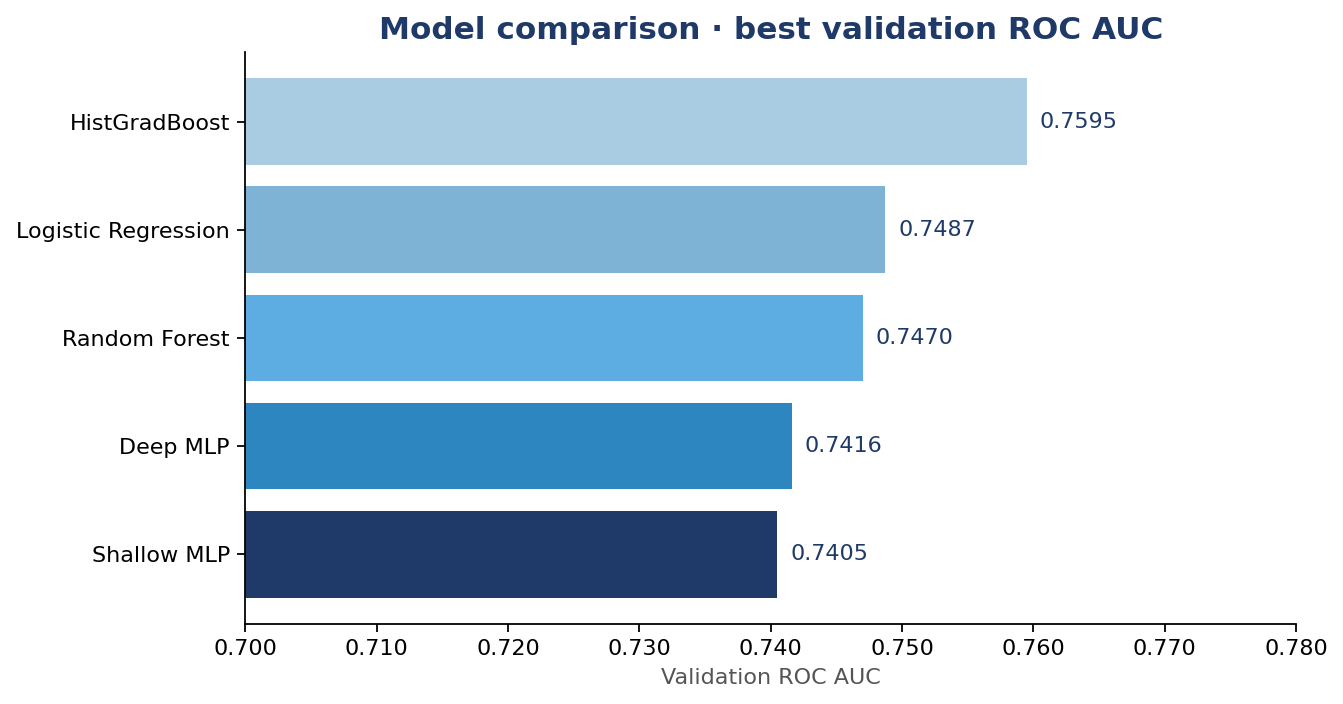
\includegraphics[width=\linewidth]{../result/home_credit/figure/model_auc_bar.png}

    \column{0.36\textwidth}
      \vspace{0.7em}
      \begin{tabular}{@{}lr@{}}
        \toprule
        \rowcolor{soft}
        \textbf{Model}  & \textbf{Val AUC} \\
        \midrule
        HistGradBoost   & \hp{\textbf{0.7595}} \\
        Logistic Reg.   & 0.7487 \\
        Random Forest   & 0.7470 \\
        Deep MLP        & 0.7416 \\
        Shallow MLP     & 0.7405 \\
        \bottomrule
      \end{tabular}

      \bigskip
      Tree boosting wins by $\sim$\hi{1 AUC point} — consistent with the literature on tabular data.
  \end{columns}
\end{frame}

% --------------------------- Slide 8 — Imbalance Handling ---------------------------
\begin{frame}{Imbalance Handling on the Best MLP}
  \vspace{0.3em}
  \begin{tabular}{@{}lcccccc@{}}
    \toprule
    \rowcolor{soft}
    \textbf{Method} & \textbf{Threshold} & \textbf{ROC AUC} & \textbf{PR AUC} & \textbf{Precision} & \textbf{Recall} & \textbf{F1} \\
    \midrule
    Baseline                 & 0.500 & 0.745 & 0.222 & 0.00 & 0.00 & 0.00 \\
    SMOTE                    & 0.500 & {\color{warn}\textbf{0.648}} & 0.134 & 0.16 & 0.21 & 0.18 \\
    \rowcolor{soft!50}
    Threshold tuning $\star$ & 0.164 & 0.745 & 0.222 & 0.24 & \hi{\textbf{0.40}} & \hi{\textbf{0.30}} \\
    \bottomrule
  \end{tabular}

  \vspace{1.1em}
  \begin{columns}[T,onlytextwidth]
    \column{0.55\textwidth}
      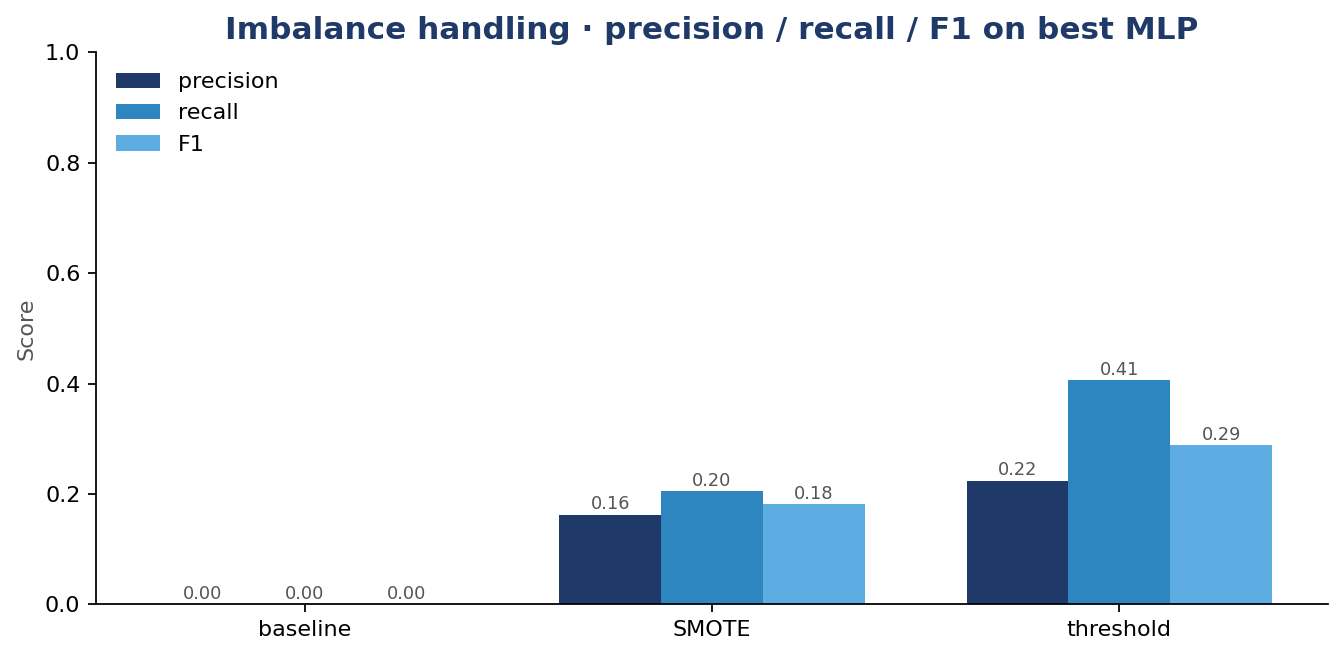
\includegraphics[width=\linewidth]{../result/home_credit/figure/imbalance_compare.png}

    \column{0.42\textwidth}
      \hp{Headline}
      \begin{itemize}\small
        \item Baseline: AUC 0.745 but recall \hi{0\%} — no prediction crosses 0.5.
        \item SMOTE \hi{hurts}: AUC dropped 0.10.
        \item Threshold tuning at 0.164 lifts recall to \hi{40\%}.
      \end{itemize}
      \medskip
      {\color{accent}\itshape Choosing the threshold matters more than rebalancing the data.}
  \end{columns}
\end{frame}

% --------------------------- Slide 9 — Conclusions ---------------------------
\begin{frame}{Conclusions}
  \vspace{0.3em}
  \hp{What we learned}
  \begin{itemize}
    \item \hi{HistGradientBoosting} wins overall at val ROC AUC $= 0.7595$.
    \item \hi{Neural networks} tie LR and RF — depth alone does not unlock new performance on tabular data.
    \item \hi{Threshold tuning} on the MLP lifts recall from 0\% to 40\%; SMOTE hurt AUC.
  \end{itemize}

  \bigskip
  \hp{Limitations}
  \begin{itemize}
    \item Only main \texttt{application\_*.csv} tables — auxiliary tables typically add several AUC points.
    \item \texttt{PredefinedSplit} is fast but optimistic; full $k$-fold CV would tighten confidence intervals.
  \end{itemize}

  \bigskip
  \hp{Future work}
  \begin{itemize}
    \item Integrate auxiliary tables  \,·\,  ensemble HGBC $+$ best MLP  \,·\,  Platt / isotonic calibration.
  \end{itemize}
\end{frame}

% --------------------------- Slide 10 — Closing ---------------------------
{
  \setbeamertemplate{frametitle}{}
  \begin{frame}
    \vspace{1.0cm}
    \begin{center}
      {\color{primary}\Huge\bfseries Thank You}\\[0.6em]
      {\color{accent}\Large Questions?}
    \end{center}

    \vspace{2em}
    \begin{center}
      \begin{tabular}{r@{\quad}l}
        \hp{Recording} & \texttt{<<INSERT RECORDING LINK BEFORE SUBMISSION>>} \\[0.5em]
        \hp{Code}      & \texttt{github.com/ymw0414/loan-default-imbalance-classification} \\[0.5em]
        \hp{Team}      & Minwoo Yoo \,·\, Nathaniel Badalov \\
      \end{tabular}
    \end{center}
  \end{frame}
}

\end{document}
